% !TEX program = pdflatex
%%%%%%%%%%%%%%%%%%%%%%%%%%%%%%%%%%%%%%%%%
% Structured General Purpose Assignment
% LaTeX Template
%
% This template has been downloaded from:
% http://www.latextemplates.com
%
% Original author:
% Ted Pavlic (http://www.tedpavlic.com)
%
% Note:
% The \lipsum[#] commands throughout this template generate dummy text
% to fill the template out. These commands should all be removed when
% writing assignment content.
%
%%%%%%%%%%%%%%%%%%%%%%%%%%%%%%%%%%%%%%%%%

%----------------------------------------------------------------------------------------
%	PACKAGES AND OTHER DOCUMENT CONFIGURATIONS
%----------------------------------------------------------------------------------------

\documentclass{article}

\usepackage{fancyhdr} % Required for custom headers
\usepackage{lastpage} % Required to determine the last page for the footer
\usepackage{extramarks} % Required for headers and footers
\usepackage{graphicx} % Required to insert images
\usepackage{subcaption}
\usepackage{lipsum} % Used for inserting dummy 'Lorem ipsum' text into the template

\usepackage[utf8]{inputenc}
\usepackage[ngerman,english]{babel}
\usepackage[T1]{fontenc}
\usepackage{breakurl}
\usepackage[hyphens]{url}
\usepackage{color}
\usepackage{float}
\usepackage[hidelinks]{hyperref}
\usepackage{tabularx}
\usepackage{enumitem}
\usepackage{color, colortbl}
\usepackage[super]{nth}
\usepackage{wrapfig}
\usepackage{amsmath}

\usepackage[
	backend=biber,
	style=numeric-comp,
	natbib=true,
	url=false,
	doi=false,
	eprint=false,
	sorting=none,
	isbn=false]
	{biblatex}

\bibliography{references}

\addto\captionsenglish{%
  \renewcommand{\contentsname}%
    {Table of Contents}%
}

% Margins
\topmargin=-0.45in
\evensidemargin=0in
\oddsidemargin=0in
\textwidth=6.5in
\textheight=9.0in
\headsep=0.25in

\linespread{1.1} % Line spacing
% Set up the header and footer
\pagestyle{fancy}
\lhead{} % Top left header
\chead{} % Top center header
\rhead{\firstxmark} % Top right header
\lfoot{\lastxmark} % Bottom left footer
\cfoot{} % Bottom center footer
\rfoot{Page\ \thepage\ of~\pageref{LastPage}} % Bottom right footer
\renewcommand\headrulewidth{0.4pt} % Size of the header rule
\renewcommand\footrulewidth{0.4pt} % Size of the footer rule

\setlength\parindent{0pt} % Removes all indentation from paragraphs

\begin{document}
\setcounter{tocdepth}{2} % No subsubsections


%----------------------------------------------------------------------------------------
% TITLE PAGE
%----------------------------------------------------------------------------------------
\pagenumbering{gobble}
% \maketitle
\begin{titlepage}
  \centering
\includegraphics[width=5cm]{figures/tumlogo}

  \vspace{2.5cm}
  \Huge{Advanced Computer Networking} \\
  \vspace{0.1in}\huge{Summary}\\

  \Large
  \vspace{1.5cm}
  \begin{tabularx}{9cm}{r l}
    Author: & Thomas Pettinger\\
  \end{tabularx}

  \vfill
  \textbf{2017--03--03} \\
  \vspace{0.3in}\normalsize{Advanced Computer Networking}\\
  \vspace{0.03in}\normalsize{\textsc{Technische Universität München}}\\
  \vspace{1cm}

\end{titlepage}
%----------------------------------------------------------------------------------------


\newpage
\thispagestyle{empty}
\tableofcontents

\newpage
\pagenumbering{arabic}

%!TEX root = ../report.tex

\section{Introduction}
Terminology:
\begin{description}
  \item[Protocols] control sending and receiving of messages
  \item[Internet] loosely hierarchical global network
  \item[Internet Standards]\hfill
    \begin{itemize}
      \item RFC:\@ Request for comment
      \item IETF:\@ Internet Engineering Task Force
      \item IANA:\@ Internet Assigned Numbers Authority
    \end{itemize}
\end{description}

\subsection{Protocols}
Protocols take care of addressing, fragmentation \& re-sequencing, error control, congestion control, compression, privacy and more.

The internet has an layered architecture of protocols.
On the sender side, protocols take the PDU (Protocol Data Unit) from layer N+1, add their header and trailer and pass the SDU (Service Data Unit) to layer N-1.
On the receiver side, the corresponding protocol takes the PDU from layer N-1, strips header and trailer again and passes the SDU to layer N+1.
\begin{figure}[H]
  \centering
  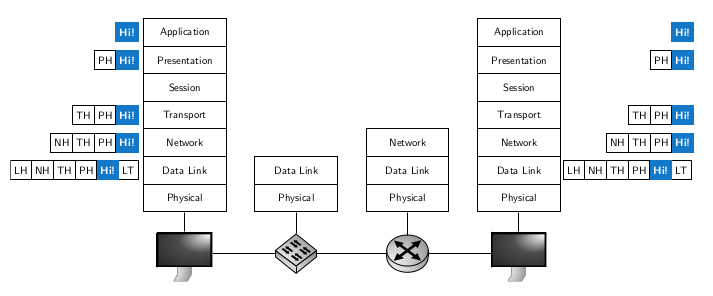
\includegraphics[width=.6\textwidth]{figures/internet_layering.png}
  \caption{Internet Layers}
\end{figure}

Protocol layering is necessary because one does not want to implement everything to the physical layer when writing a networking application.
On the other hand, layering also introduces some problems like protocol layers are sometimes reusing techniques of other layers like ARQ (Automatic Repeat Query) and layers might need informations of other layers.

\subsection{Node Forwarding Performance}
During transmission, packets might get delayed or even lost for several reasons.
First, the packets need some time to get written to router buffers, secondly the packet arrival rate might exceed the output link capacity and lastly the packets need to wait again for being sent from the packet queue in routers.

The sources for these delays are listed below.
\begin{enumerate}
  \item Processing delay: interrupt handling when receiving new packets and processing for further transmission
  \item Queuing delay: waiting time in output queue
  \item Transmission delay: time to send bits into link: $= \frac{\text{packet length L (bit)}}{\text{link bandwidth (bps)}}$
  \item Propagation delay $=\frac{\text{length of physical link d}}{\text{propagation speed} \approx 2 \cdot 10^8 m/s}$
\end{enumerate}
The total amount of delay is then $d_{nodal} = d_{proc} + d_{queue} + d_{trans} + d_{prop}$

To reduce total packet delays for a connection consisting of several links one can use circuit switching, where packets do not have to be received entirely to be sent to the next link.
Another alternative is to split packets into (very) small sub-parts (= segmenting) and using pipelining (parallel computing of packets).

\newpage

%!TEX root = ../report.tex

\section{Link Layer}

\newpage

%!TEX root = ../report.tex

\section{Network Layer}
The network layer serves the following functions:
\begin{itemize}
  \item IP protocol for addressing, datagram format and packet handling conventions
  \item Routing protocols for path selection
  \item ICMP protocol for error reporting and router signaling
\end{itemize}

\subsection{Internet Protocol}
\begin{figure}[H]
  \centering
  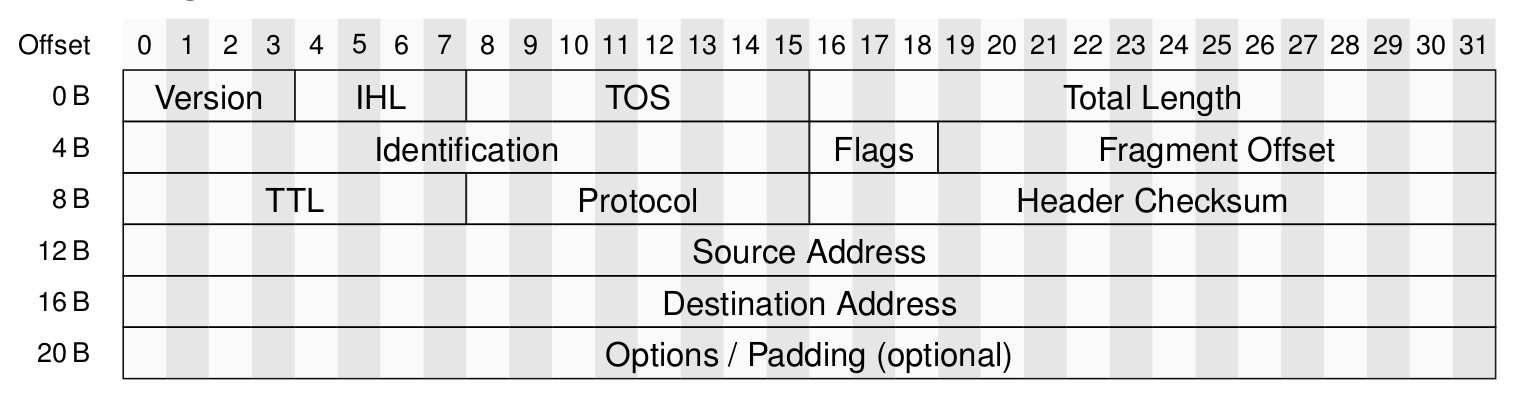
\includegraphics[width=.8\textwidth]{figures/ipv4_datagram.png}
  \caption{IPv4 Datagram}\label{fig:ipv4_datagram}
\end{figure}

\subsubsection*{IPv4 Addressing}
IPv4 addresses are 32-bit identifiers for every host and router interfaces where interfaces represent the connection between host/router and physical link.

Subnets are device interfaces with the same subnet part of the IP address which can physically reach each other without intervening router.

Splitting the IP address into network and host part is done in the following way (for the address 192.168.128.1/17):
\begin{figure}[H]
  \centering
  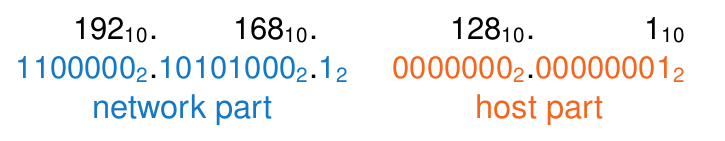
\includegraphics[width=.6\textwidth]{figures/ip_split.png}
\end{figure}

From 1982 to 1993, IP addresses were classfully divided as shown in Figure~\ref{fig:classful_ips}.
\begin{figure}[h]
  \centering
  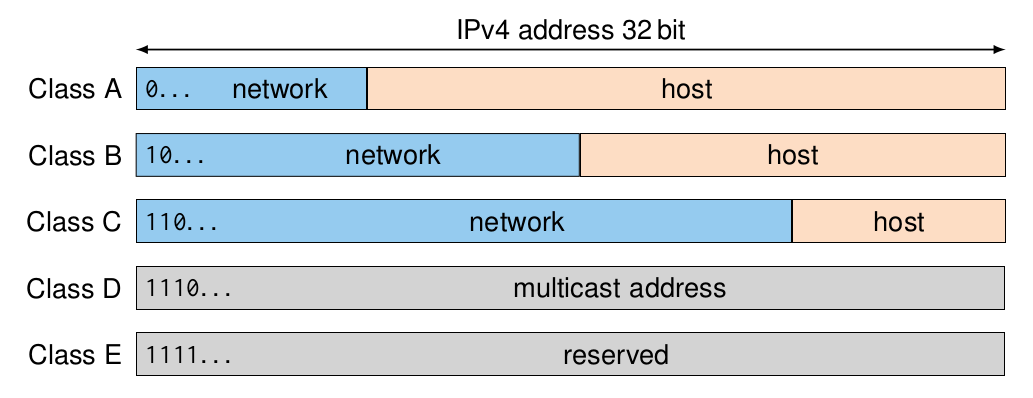
\includegraphics[width=.8\textwidth]{figures/classful_ip.png}
  \caption{Classful IPs}\label{fig:classful_ips}
\end{figure}
In 1993, Classless Inter-Domain Routing (CIDR) was introduced which allowed arbitrary subnet length.
To route packets, prefix matching is used which checks which entry in the routing table fits best for the incoming packet's network prefix.

\subsection{ICMP}
The Internet Control Message Protocol (ICMP) are located above IP but can be considered as part of the IP layer.
It is used for communicating error messages and other attention requiring conditions for IP and TCP or UDP\@.
Two classes of ICMP messages are possible:
\begin{enumerate}
  \item Query messages: only kind that generates other ICMP messages
  \item Error messages: contain IP header and first 8 bytes (today as much as possible up to 572 bytes) of datagram that caused the ICMP message which allows the receiver to put it into context
\end{enumerate}
The structure of an ICMP message is shown in Figure~\ref{fig:icmp_message}.
\begin{figure}[H]
  \centering
  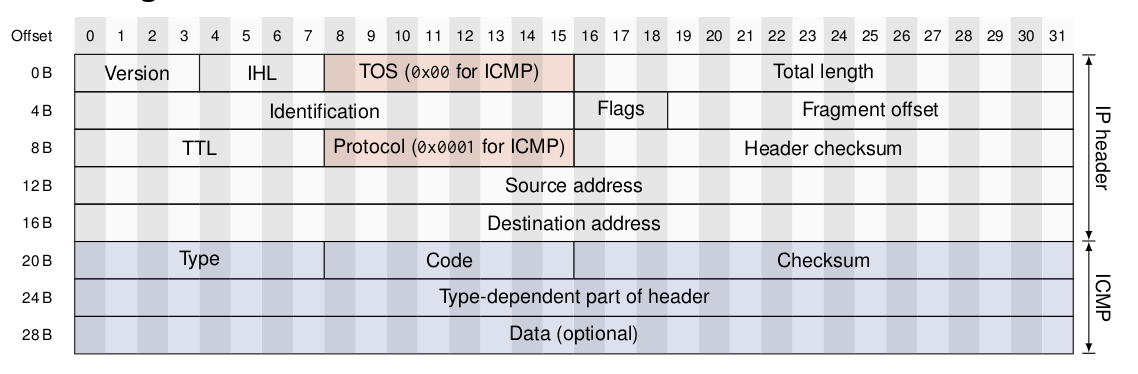
\includegraphics[width=.8\textwidth]{figures/icmp_message.png}
  \caption{ICMP Message}\label{fig:icmp_message}
\end{figure}


\newpage

%!TEX root = ../report.tex

\section{Structure of the Internet}
The Internet is separated into regions called \textbf{autonomous systems (AS)}.
Routers in the same AS use \textbf{intra-AS routing} protocols whereas routers connecting different ASes, called \textbf{gateway/border routers} use \textbf{inter-AS routing} protocols.
\textbf{Transit domains} are ASes, that forward traffic from one AS to another where in contrast a \textbf{stub domain} is an AS without transit traffic.
Internet service providers are divided hierarchically: Tier-1 providers are on the top level and connected to each other.
They can send traffic to one another without paying (peering).
Tier-2 providers are connected to one or multiple Tier-1 providers and possibly to other Tier-2 providers.
Tier-3 providers and local ISPs then are the last hop to the end systems.
Every ISP has its own IP range purchased at the regional Internet Registrars which they are able to divide amongst their customers.

\subsection{Associations of Internet Names and Numbers}
\begin{description}
  \item[ICANN] Internet Corporation for Assigned names and numbers: Administration of DNS TLDs
  \item[IANA] Internet Assigned Numbers Authority: Assignment of Internet Numbers, administration of DNS root name servers and reverse DNS infrastructure, Assignment of protocol names and numbers
  \item[NRO] Number Resource Organization: Association of the 5 Regional Internet Registrars (RIR)
  \item[Regional Registras] Assigns IP addresses and AS numbers, administration of local Internet Registers (LIR)
  \item[RIPE] Registration and administration of Internet resources: AS, prefix and routing information
\end{description}

\subsection{Routing Algorithms}
Routing algorithms are usually an applied approach of least-cost path search in weighted graphs.
The costs are represented for example by the inverse link bandwidth.

They can be classified by several criteria:
\begin{itemize}
  \item Global or decentralized
  \begin{itemize}
    \item Global/Link State algorithms (L-S): All routers know the graph topology and link costs (usually through broadcasts) and are able to calculate the routing table by themselves (usually via Dijkstra)
    \item Decentralized/Distance Vector algorithms (D-V): Routers only know neighbours and link costs to neighbours, routing tables are computed in collaboration
  \end{itemize}
  \item Static or dynamic
  \begin{itemize}
    \item Static: Routes change slowly over time
    \item Dynamic: Routes change more quickly due to periodic update and in response to link cost changes
  \end{itemize}
  \item Scope: Intra- vs Inter- vs special purpose
  \item Type of traffic: Unicast vs multicast
  \item Trigger type: permanent routing vs on-demand routing (create routing table only if necessary)
\end{itemize}

\subsubsection*{D-V Algorithm}
A typical example for a distance vector algorithm is the Bellman-Ford algorithm:
\begin{enumerate}
  \item Define $D_x(y)$ as the estimate of the least cost from x to y
  \item Node x knows all costs to each neighbour v: $c(x,v)$
  \item Every node x maintains a distance vector $D_x = [D_x(y): y \in N]$ where N is the set of nodes
  \item Node x also maintains the distance vectors for each neighbour $D_v = [D_v(y): y \in N]$
  \item Update messages for the estimated distances are sent from time to time to neighbours and might lead those to update its own distance vectors according to the B-F equation:
    $D_x(y) \leftarrow \min_v{c(x,v) + D_v(y)} \text{ for each node } y \in N$
  \item Under minor, natural conditions these estimates of $D_x(y)$ to the actual least costs $d_x(y)$
\end{enumerate}

A problem which occurs with this approach is that if a link becomes unavailable and thus its cost infinity, the algorithm will encounter the count to infinity problem.
The paths to the disconnected node are increased per update by one, infinitely.
Solutions for this are
\begin{itemize}
  \item Finite infinity: set infinite costs to a specific number, e.g. 16 in RIP
  \item Split Horizon: Tell neighbours that they are part of the best path to a destination that the destination cannot be reached from the original node
  \item Poisoned Reverse: Actively adverse a route as unreachable to neighbours from which the route was learned
\end{itemize}

\subsubsection*{Path Vector Protocols}
Path vector protocols try to improve the fact of D-V protocols that they do now include topology information.
For each destination, the entire path for each destination is told to neighbours and then the cost calculation is done by looking at the paths.
Furthermore loop detection can easily be done by searching if the own node ID appear in the paths.
PV protocols are quite rarely used though, mainly in BGP but that is much more complex than just paths.

\subsubsection*{Intra-AS Routing/Interior Gateway Protocols (IGP)}
\begin{enumerate}
  \item RIP: Routing Information Protocol
  \item OSPF: Open Shortest Path First (hierarchical LSA), usually in medium to large systems
  \item IS-IS: Intermediate System to Intermediate System, medium-sized ASes
  \item (E)IGRP: (Enhanced) Interior Gateway Routing Protocol, CISCO proprietary, hybrid of LS and DV
\end{enumerate}
\vspace{5pt}

The open shortest path first protocol (OSPF) uses an link state algorithm to generate routing tables.
Advertisement of topology and costs of the directed graph is done via advertisement flooding.
All messages are authenticated to prevent malicious intrusion (e.g.\ with IPsec).
Furthermore multiple same-cost paths are supported and different metrics are considered to define the costs for links.
The protocol has integrated unicast and multicast support (Multicast OSPF) that uses the same topology database as OSPF which lowers traffic.
To even further reduce the traffic, hierarchical OSPF can be used in large domains where a two-level hierarchy is created.
On the one side the backbone which are running OSPF among themselves and on the other hand local areas.
Area border routes summarize distances to networks in the own area and advertises them to other area border routers.

\subsubsection*{Inter-domain routing}
Inter domain routing is almost exclusively handled with the Boarder Gateway Protocol (BGP).
It provides means to obtain subnet reachability from neighbouring ASes (external BGP, eBGP), propagate that information in the AS internally (internal BGP, iBGP) and determine good routes according to that information and router policies via semi-permanent TCP connections.
ASes advertise reachable network prefixes to others and give a promise to forward traffic to that IP address space.
These advertisements include a multitude of BGP attributes like AS-Paths (Path of AS-Numbers the advertisement has passed through) or the Next-Hop (gateway router to the next-hop AS).

BGP messages can have the following types:
\begin{itemize}
  \item OPEN: open a BGP session
  \item NOTIFICATION: error occurred, close BGP session
  \item KEEPALIVE: null data to prevent closing of TCP session
  \item UPDATE: about changed routes, also removed routes\\
    These messages consist of the destination IP prefix, the AS path and the next hop and other attributes related to local preferences, route origins or others.
    Routers than can make routing decisions based on this information and their policies.
\end{itemize}

Routers may learn about multiple routes for a prefix.
If that is the case, one of those routes has to be selected due to criteria like an policy decision, shortest AS-Path or closest next hop (hot-potato-routing) amongst others.\\
\vspace{5pt}

In the context of inter-domain routing, we define the following \textbf{terminology}:
\begin{description}
  \item[Transit AS] Relays traffic between other ASes
  \item[Stub AS] Buys transit from one other AS but does not offer transit
  \item[Multi-homed AS] Buys transit from $\geq 2$ other ASes, does not offer transit
  \item[Peering] having a BGP relationship
    \begin{itemize}
      \item Private peering: peering between ASes in private locations like ASes or neutral server rooms
      \item Public peering: "official" peering locations ("Room full of switches") like in Frankfurt or London
    \end{itemize}
  \item[Provider] Offers transit traffic for receiving money
  \item[Customer] Gets transit for paying money
  \item[Siblings] Mutual transit agreement to provide connectivity of the rest of the Internet for each other, so kind of an very extensive peering
\end{description}

\subsubsection*{Business and Policy Routing}
Routing is done by the policy
\begin{equation*}
  \text{Routes via customer > Routes via peer > routes via provider}
\end{equation*}
In route announcement on the other hand first announce routes that incur financial gain if others use them, then routes that reduce costs if others use them and especially do not advertise routes that incur financial loss as long as an alternative exists.
ASes might add the same AS number subsequently to an AS-Path to increase path costs if they prefer another connection over the one this announcement was sent, might be due to lower costs.

\subsubsection*{Tiers and Default-Free-Zone}
Like mentioned in the introduction to this chapter, different tiers of providers exist.
With our definitions in inter-domain routing of costumers, providers and peering, we can now better define them:
\begin{description}
  \item[Tier-1/Default-Free-Zone (DFZ)] Only have customers and peers, no providers
  \item[Tier-2] only peerings and only tier-1 providers
  \item[Tier-n] at least noe tier-(n-1) provider
\end{description}

\subsubsection*{Internet Fixed Points}
Internet fixed points are ASes that are stable over a long period of time from different perspectives.
Together these form the so called backbone of the Internet.
To find those fixed points, the \textbf{k-core algorithm} can be applied:
\begin{enumerate}
  \item Remove all nodes with $degree = 1$ so long until no degree 1 nodes are left
  \item Remove all nodes with $degree = 2$ so long until no degree 2 nodes are left
  \item Do this until no nodes left $\Rightarrow$ $(Steps - 1)-core$ found.
\end{enumerate}

\newpage

%!TEX root = ../report.tex

\section{Network Measurement}
Network performance can be measured for different metrics like throughput (bandwidth or packet rate), latency (average, median, standard deviation,\dots), frame loss rate, topology measurements or others with different circumstances (load, traffic type,\dots).
Different RFC standards exist as guideline.

\subsection{Throughput}
Throughput is usually limited by the line rate and the speed and size of the lookup tables.
It is measured in packets per second (not bandwidth) since routers usually only look at packet headers and not the entire packet, so the actual size has only a minor importance.
The worst case scenario regarding costs is network traffic at line rate and minimum packet size which is the minimum sized Ethernet packet plus the 7 byte preamble, 1 byte start-of-frame delimiter and the minimum inter-packet gap of 12 bytes, thus 84 bytes.\\
\vspace{4pt}

When testing, different measuring methodologies can be applied.
The simplest one is to apply the highest possible packet rate on A and measure the packet rate at B.
With this method, the devices might get overloaded though which leads to different behaviors.
So a better version is to apply varying rates on A and find the highest rate were no loss occurs (RFC 2544).
Problems of this approach again are that some devices loose packets when suddenly facing high packet rates due to energy saving mechanisms.
As a summary the best approach depends on the device under test.

\subsubsection*{Improving Throughput}
Potential bottlenecks for packet forwarding are CPU processing power, NIC processing power, Bus bandwidth, memory bandwidth or CPU caches.
As researches found out, the biggest limitation origins in the CPU.
The most time is spent to process, receive and transmit packets there.
When transferring the network stack from kernel to user space, performance can be significantly increased due to fewer expensive system calls, simplified memory management and batch processing through the whole application.
The disadvantages on the other hand are that only raw packets are handled, so protocols have to be reimplemented for every application, NICs can only be used by one application and there is no API compatibility to traditional user space applications.

\subsection{Parallel Packet Processing}
Modern NIC cards hare configurable to use multiple rx and tx queues to support multi-core parallelization to improve performance.
Several metrics to distribute incoming traffic on the queues exist:
\begin{itemize}
  \item Per-packet basis: Slow when protocol state has to be synchronized and might cause packet reordering
  \item Per-flow basis: Fast, protocols handled in the same core and cache and prevents packet reordering
  \item Explicitly: Useful for e.g. virtual machines, slower than flow-based though
\end{itemize}
Usually packet forwarding is done in kernel space due to better performance than the socket API.

\subsection{Latency}
Sources of latency are serialization, propagation and calculations where buffers usually are the biggest bottleneck.
Also the technique to receive packets plays a role:
\begin{itemize}
  \item one interrupt per packet: low latency but also low throughput because interrupts are expensive
  \item one interrupt for multiple packets: high throughput but also high latency
  \item no interrupts but polling based: low latency and high throughput but inefficient at low packet rates (busy waiting)
\end{itemize}

\subsection{Packet Generators}
Packet generators exist in hardware and software varieties.
Hardware generators are fast, precise and accurate.
Software ones run on cheap hardware and are very flexible but face challenges with rate control and time stamping.\\

To control the packet rate software implementations push single packets to the NIC where queues cannot be used.
Also the NICs work with asynchronous push-pull models which can lead to micro bursts and thus to unreliable, imprecise and bad performance.
Hardware generators on the other hand support hardware rate control where queues can be used and have good performance but they are quite inflexible.
To combine the advantages of both, one can disable hardware control and use invalid packets in the queues to control the rate since those are simply dropped by the device under test without much overhead.

\subsection{Internet Wide Scans}
When doing larger scale network scans are performed, several points have to be taken into consideration.
For one which targets are selected which might be a specific hitlist provided by e.g.\ traceroute, web server logs or traffic traces, certain IP addresses per subnet or even a full 0/0 scan.
Also there are performance requirements that need to be met and ethical considerations, too, since one causes sometimes large amounts of traffic on the scanned network.\\
\vspace{4pt}

\subsubsection*{Nmap}
Nmap is a common measurement tool which provides host discovery, service detection, OS detection and support for custom scripts.
It provides a multitude of scanning techniques:
\begin{itemize}
  \item TCP scan: Sends TCP packets with different flags set. A SYN scan checks for open ports, ACK scans scan for (un-) filtered ports by a firewall. Some more exist.
  \item ICMP scan: ping requests
  \item UDP payload scan: Sends UDP packets with different payloads
\end{itemize}
While scanning, randomization is used to avoid complaints of system administrators but only groups of 16k hosts are possible.
Nmap uses a stateful scanning approach to keep track of every packet in transit and to catch timeouts to try again to send packet.\\

\subsubsection*{Zmap}
A full Internet scan using nmap takes around 10 days which is quite slow.
For that reason, \textbf{zmap} was developed by the university of Michigan which is able to do a full scan in around 45 minutes.
It uses TCP SYN or UDP payload scans to find open ports and it is possible to distribute the scanning load on different machines and every IP is only scanned once.
The performance is reached by using raw sockets and not keeping state of packets which makes it impossible to detect timeouts though.
This is handled by cycling through the host IPs that have not jet responded a certain amount of times and then abort.
Furthermore without keeping states, incoming packets that belong to the scan are more difficult to identify.
Zmap therefore uses IP IDs which are used to generate a validation with AES which is stored in the packet sent e.g.\ in the sequence number
When receiving packets, they are validated using the validation, in the example from before $sequence~number- 1$.

\subsubsection*{IPv6 Scanning}
IPv6 scanning faces different challenges than IPv4 due to different routing, firewall and host configuration and the huge address space.
To to the amount of possible addresses it is not possible to do a 0/0 scan so hitlists are used to define the targets.
Sources for such hitlists are for example the Alexa Top 1 Million list (most popular websites), the Rapid7 DNS ANY list or DNS zone files (content of TLD name zones).
Also traceroute or passive sources like packet traces or flow data can be taken into account.\\
\vspace{4pt}

IPv6 scans can be evaluated for reachability or stability.
Also as long as the targets do not use IPv4 privacy extensions (Interface ID randomly chosen) the target device type can be determined.
The criterion is that routers usually have the IID ::1 for the default gateway.

\subsubsection*{Security Scans}
\textbf{TLS scans} are used to scan the state of TLS protocols like HTTPS or IMAPS in the Internet by analysing certificate chains, expiry and algorithms.
Scans are done by identifying hosts that offer TLS services, download the certificate chains and analise and validate these chains.\\
\vspace{4pt}

\textbf{SSH scans} mainly provide an overview over the security of the SSH configurations of hosts with public IPs.
Since SSH is mostly used for administrative or security sensitive contexts it is usually advisable to notify CERTs, watchlist services and blocklist operators about scans.
Also other measurements like an own scanning subnet with a abuse WHOIS email contact might be useful to hide one's identity.\\
In the past several internet wide SSH scans were performed which analysed key strength (length, debian weak keys, duplicate keys).\\
\vspace{4pt}

\textbf{IPMI (Intelligent Platform Management Interface)} is a out-of-band management system used in servers.
It uses a separate OS which has full access to the host OS\@.
IPMI scans try to detect known vulnerabilities in configurations, i.e.\ hosts should not be reachable from the public internet.
When combining IPMI responses with HTTPS reachability to detect IPMI web-interfaces which also might be vulnerable.
Compromised web servers again may lead to a compromised OS.\\
Internet wide scans for IPMI-over-IP devices are showing declining numbers of reachable devices.
Those who are reachable are heavily clustered in a view ASes though and detected HTTPS interfaces show that 90\% of them have 1024 bit or shorter keys.\\

\textbf{BACnet (Building Automation and Control Networks)} is a protocol that is used to control heaters, solar panels and other building automation aspects.
Access to those systems can lead to real world consequences.
It is based on UDP and has no build in security.
Devices providing this protocol have properties that can be queried via a SingleProperty or MultipleProperty request which enables attackers to generate larger responses which results in easier DOS attacks.
To detect these easily possible attacks, scans are performed to check the BACnet deployment in the internet.

\subsubsection*{Ethical considerations}
It is usually advisable to take some ethical steps before doing Internet wide scans.
These include reducing the intrusiveness of scanning by avoiding logins or limit the scanning rate, providing information on the scanning machine's website, respond quickly to every inquiry and abuse email and offer possibilities for blacklisting IPs.
A general guideline here is to be the "nice guy".

\subsection{Passive Measurements}
Passive network measurement does not cause additional traffic like the approaches mentioned above but uses monitoring probes to analyze existing traffic.
Important metrics here are traffic volume, traffic composition and packet inter-arrival times with different levels of granularity.
When captured, different analyses can be performed, e.g.\ network utilization, QoS parameters, detection of failures and anomalies or traffic characterization.
These informations might be useful for accounting, security or traffic engineering.\\

The capturing hardware usually has to be able to perform on multi-gigabit/s links with relative cheap costs and simple deployment.
Common approaches to these requirements are high-end network adapters with large amount of memory and functionality (still cheap?), sophisticated algorithms by eliminating copying of packets amongst others, sampling (probabilistic filtering of packets), filtering (mask, router state, hash based) and aggregation.\\

The process passive measurement is depicted in Figure~\ref{fig:passive_network_measurement}.
\begin{figure}[h]
  \centering
  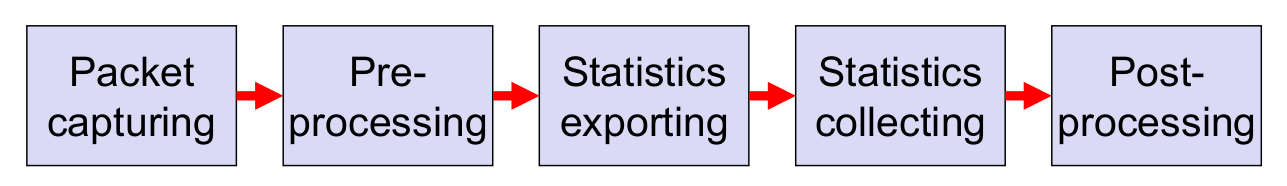
\includegraphics[width=.8\textwidth]{figures/passive_network_measurement.png}
  \caption{Passive Network Measurement Process}\label{fig:passive_network_measurement}
\end{figure}

\textbf{Packet capturing} is assisted by hardware.
Server NICs have direct access to the main memory without processor support and do batch processing to reduce copy operations.
Also special monitoring interface cards exist which usually only are able to receive data and provide certain processing features like filtering, high-precision time-stamps and others.

\subsection*{Flow-based Traffic Measurements}
Flows describe packets which belong together like all packets of a TCP connection (IP-5-Tuple).
Flow data is usually measured passively on the network and is exported when on of two timeouts runs out.
The inactive timeout starts at the last received packet of a flow and is reset with every packet.
The active timeout starts with the first packet of a flow and is only reset if it expires.
The inactive timeout was designed to export flow data of short lived flows whereas the active timeout sends data during a flow is active for long lived ones.

\subsubsection*{IP Flow Information eXport (IPFIX)}
The IPFIX protocol was defined by the IETF in RFCs and is an extensible flow exportation protocol.
The extensibility is achieved by differentiating between template and data records where the template defines the data format for the data records.\\
During measurement, statistical counters and values are updated and whenever a flow terminates, the data is exported via SCTP or, if available, TCP or UDP.\\
The metering process of IPFIX includes packet header capturing, timestamping, classifying and the maintaining of flow records where a flow record contains information about measured properties of the flow like total number of bytes in the flow or IP addresses.
Exporting then sends flows to one or more collecting processes.
In the end data is collected from all capturing points and further processed.\\
Metering and exporting can be done on network devices directly, or be on separate hardware.
Collecting is usually done separately.\\
Sampling and filtering can be used for very high-speed networks.

\subsubsection*{Anomaly Detection with Machine Learning}
Machine Learning can be used to detect anomalies based on flow data.
For this, feature vectors have to be created from flow data with numerical and categorical semantics.
An example for such a transformation of the data is shown in Figure~\ref{fig:ml_feature_vector_creation}.
\begin{figure}[h]
  \centering
  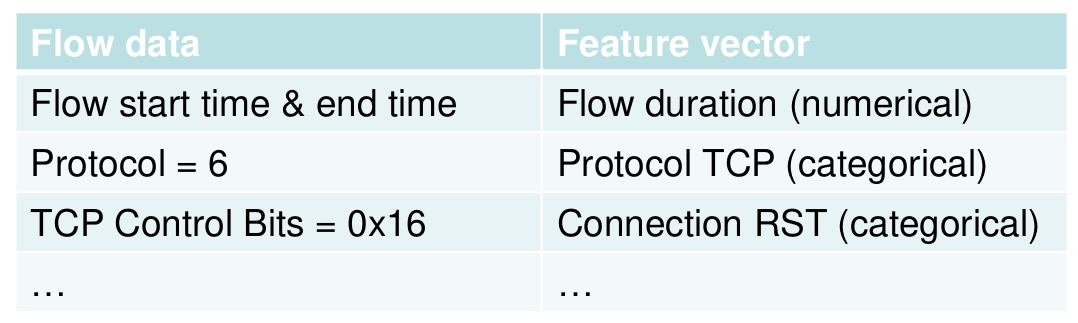
\includegraphics[width=.7\textwidth]{figures/ml_feature_vector_creation}.
  \caption{Feature Vector Creation}\label{fig:ml_feature_vector_creation}
\end{figure}

\textbf{Supervised machine learning} then uses labeled training data to learn what is benign and malicious traffic.
\textbf{Unsupervised ML} on the other hand has no training data available.
It tries to find clustered data and outliers.
The outliers then represent an anomaly.\\

To assess the quality of these approaches, different metrics can be used:
\begin{itemize}
  \item Precision = $\frac{\text{true positives}}{\text{true positives + false postives}}$\\
    How many of the detected anomalies are actual anomalies?
  \item Recall = $\frac{\text{true positives}}{\text{true positives + false negatives}}$\\
    How many of all actual anomalies did I detect as anomalies?
  \item Accuracy = $\frac{\text{true positives + true negatives}}{\text{all}}$\\
    How many positive and negative classifications are correct?
\end{itemize}
The goal is to decrease false positives and negatives here, but in reality decreasing on type of error increases the other.

\subsection{Amplification Attack Detection}
In amplification attacks, the attacker sends small request to an amplifier network with a spoofed IP address which generate large response packets to the victim (owner of the spoofed address).\\
The amplifier network might be able to detect such an attack though by passively measuring incoming and (potential) outgoing traffic.
Different characteristics can be used then to identify an attack:
\begin{itemize}
  \item Amplification factor: compare incoming and outgoing traffic, if asymmetric an attack is possible
  \item Packet size similarity: Same sized packets incoming frequently
  \item Payload similarities: Packets from the attacker have similar payload content. Payload similarities are detected by a low entropy.
  \item Unsolicited ICMP messages: backscatter ICMP message of the victim are indicator for an attack
  \item TTL measurements: path form attacker $\neq$ path from amplifier to victim indicates an attack
\end{itemize}

\subsection{Hybrid Measurements}
A hybrid approach between active and passive measurement can be taken where packet flows are modified by piggybacking or header modification.
This enables adding additional information to packets without applying additional load to the network.
This has to be taken with care though, since people might not like this.

\subsection{Detecting Traffic Misdirection in Interdomain Routing}
\begin{figure}[H]
  \centering
  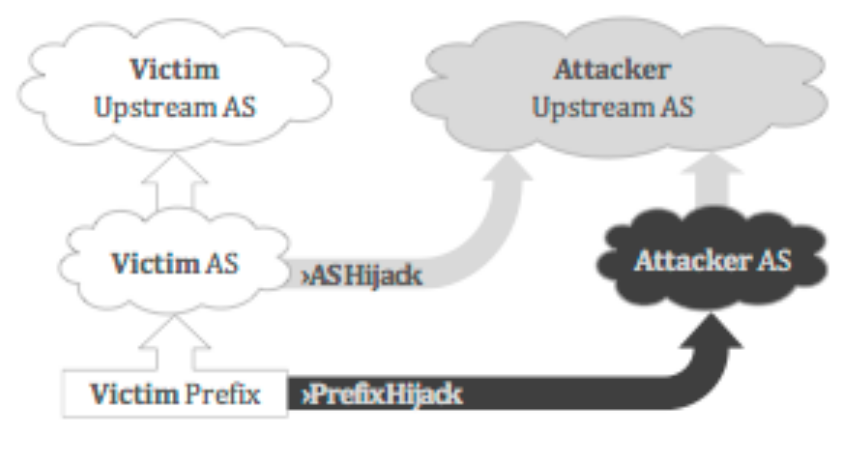
\includegraphics[width=.6\textwidth]{figures/as_and_prefix_hijacking.png}
  \caption{Possible attacks}\label{fig:fig:as_and_prefix_hijacking}
\end{figure}

In prefix hijacking attackers announce a victim's (sub-) prefix to other ASes.
We already have real-time detection for that.
AS Hijacking is a more sophisticated approach where a letter of authorization has to be accepted by ISPs as a legitimation to advertise resources of a customer's AS\@.
Such an attack is usually carried out over several month.
In the example of LinkTel, the attackers re-registered an expiring domain (link-telecom.biz), forged an letter of authorization to the upstream provider and announced false BGP routes.\\
In 2013 an escalation warning system for AS hijacking was designed at the TUM which uses passive monitoring of DNS expiry an re-registration and analysis of reverse DNS and BGP activity to identify vulnerable targets.

Current hijack detection is done via multiple traceroute scans from multiple vantage points.
To identify the poisoned part of the network, last hops to the target prefix and downstream graph of last hops are regarded.
Possible detection metrics are a detection of an odd distribution of first-rank countries (5 neighbours Germany, 1 New Zealand), an odd distribution of first-rank ASes or odd RTTs.
Also Exclusive AS connectivity can be used to detect how many ASes in the graph are connected exclusively through one neighbour of the target.
With that approach a segmentation of the graph is possible which allows the specification of the impact of a possible hack.\\

\newpage

%!TEX root = ../report.tex

\section{Software Defined Networking}
Traditional networking has the problem that distributed connectivity algorithms do often times not find the best solution (e.g. spanning tree protocol) and scenario-specific requirements are generally hard to implement.
Furthermore due to the lack of abstraction, it is hard to manage a network and the innovation is slow.
Theses problems are tried to be solved by software defined networking.\\
\vspace{5pt}

The idea behind SDN is to have the control plan logically separated from the forwarding plane so that is handled centrally.
This way, the central control point can be used to calculate spanning trees or load balancing and thus render worse distributed algorithms unnecessary.
Furthermore the forwarding behavior can be specified more precisely, e.g.\ forbidding traffic from one VM to another and an higher level of abstraction can be introduced by adding a API level between hardware devices and control plane.
This abstraction greatly increases the speed in which the forwarding logic can be modified since instead of having to buy new hardware that all speak the same protocol, only some software changes have to be made.
The actual forwarding plan then only executes the specified behavior of the control plane.
Figure~\ref{fig:sdn_big_picture} shows the model of SDN.
\begin{figure}[h]
  \centering
  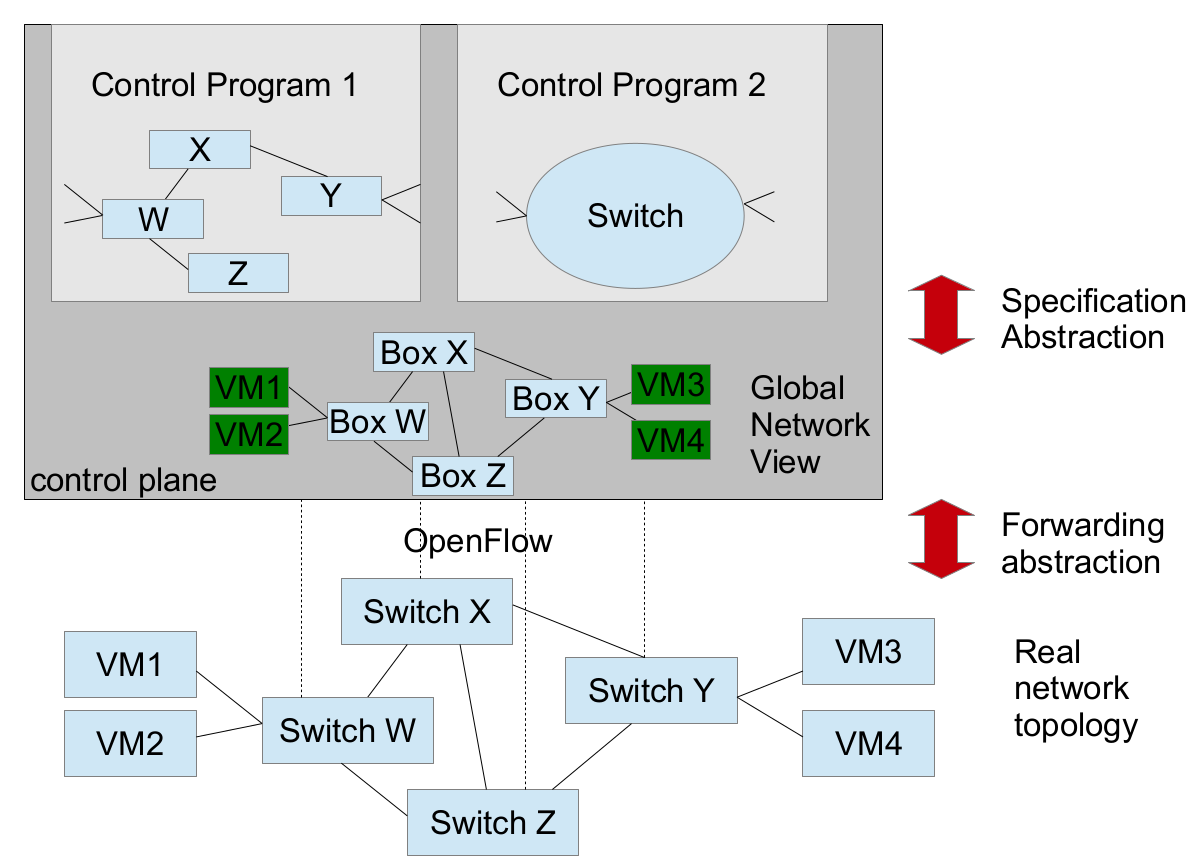
\includegraphics[width=.6\textwidth]{figures/sdn_big_picture.png}
  \caption{SDN big picture}\label{fig:sdn_big_picture}
\end{figure}

\subsection{Network Operating Systems}
A network operating system like for example OpenFlow manages network hardware, provides SDN control plane services and provides a standardized API to hardware resources.
Figure~\ref{fig:network_operating_system} shows the abstractions in a NOS.
\begin{figure}[h]
  \centering
  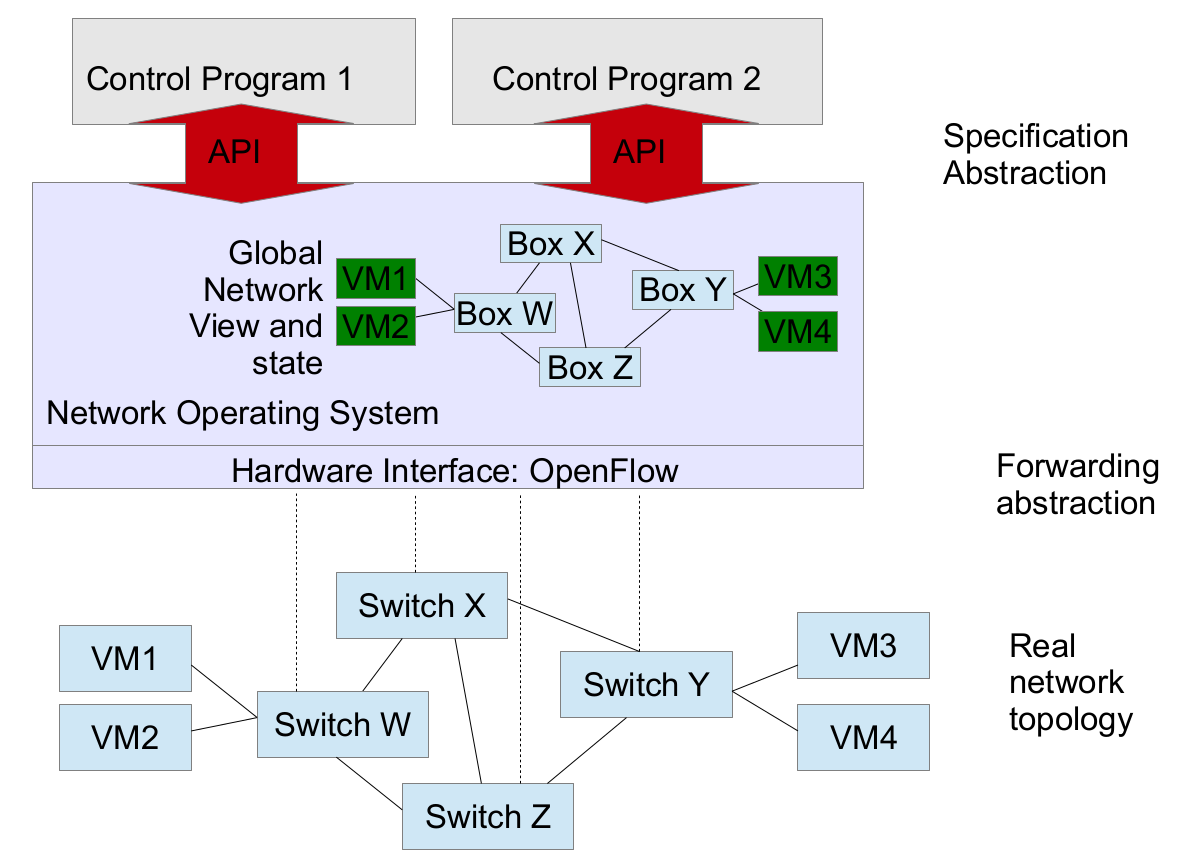
\includegraphics[width=.6\textwidth]{figures/network_operating_system.png}
  \caption{Network Operating System Model}\label{fig:network_operating_system}
\end{figure}
With an NOS we have a central control plane which handles the difficult network and routing computations.
This way the actual forwarding switches are only "dumb boxes" which are connected via ssl to the NOS which runs on fairly common CPUs.

Some disadvantages of SDN are that more configuration is required than in traditional forwarding and a single point of failure exists.

\newpage

%!tex root = ../report.tex

\section{Quality of Service}
Quality of service are performance guarantees given to customers in a service level agreement (SLA).
These performance guarantees might be important for different scenarios like streaming, interactive applications (games,\dots) or safety-critical application or safety-critical applications.
SLAs are applied at different levels: packet, flow, application or user level.
To guarantee the specifications in an SLA one has to perform different tasks:
\begin{itemize}
  \item Modelling: Understand which parts of the network have an impact on the SLA\\
    These usually are propagation, processing, transmission and queuing delay.
  \item Classification: Identify which packet need SLA\\
    Several methods exist for identification like using packet header fields like IP-5-Tuple or IPv4 TOS field or another alternative is to do deep packet inspection.
  \item Scheduling: Give preferential service to network packets.
    Two types of schedulers can be differentiated: work-conserving schedulers only are idle if no packet available whereas non-work conserving ones might be idle even if packets are pending.\\
    The common architecture for scheduling is to have multiple queues with different priorities.
    The queues are pulled if all queues with higher priority are empty.\\
    A slight deviation of this approach is round robin, where the queues are polled after one another.\\
    A third approach namely \textbf{weighted fair queuing} tries to solve the problem of round robin queueing, where the bandwidth per queue depends on the packet sizes, and priority queue scheduling (starvation) by splitting the actual available bandwidth according to the weights of different queues.
    The implementation is much more complex though and thus it is rarely used in real switches.
  \item Monitoring: Check actively or passively if SLAs are met.\\
    This can be done with live tests, emulations or simulations or formal verification methods.
    The more critical real-time requirements an application has, the more precise the measuring algorithms typically are.
\end{itemize}

\subsection{Deterministic Network Calculus}
Network calculus is a framework developed for analyzing performance guarantees in networks of queues and schedulers.
In the deterministic variant, no randomness is involved whereas the stochastic model includes randomness and thus is characterized in probabilistic terms.\\
Packets and network protocols are described as \textbf{flow}, meaning an unidirectional set of packets going from a sender to a receiver and are modeled by a \textbf{cumulative arrival function} A.
$A(t)$ represents the amount of data sent by the flow in the time interval $[0,t)$.The 
The \textbf{deterministic arrival curve} then is defined as $A(t) - A(s) \leq \alpha (t-s), \forall 0 \leq s \leq t$.
A simple example for this would be the \textbf{token bucket} $y_{r,b}(t,s) = r \cdot (t-s) + b$ where r denotes the average rate and b the burstiness parameter.\\
Queues and schedulers are seen as \textbf{servers} in network calculus.
They have a \textbf{deterministic service curve $\beta$} such that the output curve $A^* \geq \inf_{0 \leq s \leq t} \{A(s) + \beta (t-s)\}$
A simple example for this is the \textbf{rate-latency} which is defined as $\beta_{R<T}(t) = R[t - T]^+$ where R is the rate, T the processing delay and $[x]^+ = max(0,x)$.\\
Delay is defined as time time it takes for a packet to traverse the queue and queue size as the backlog size at the server.
For a visualization see Figure~\ref{fig:nc_delay_and_backlog}.
\begin{figure}[h]
  \centering
  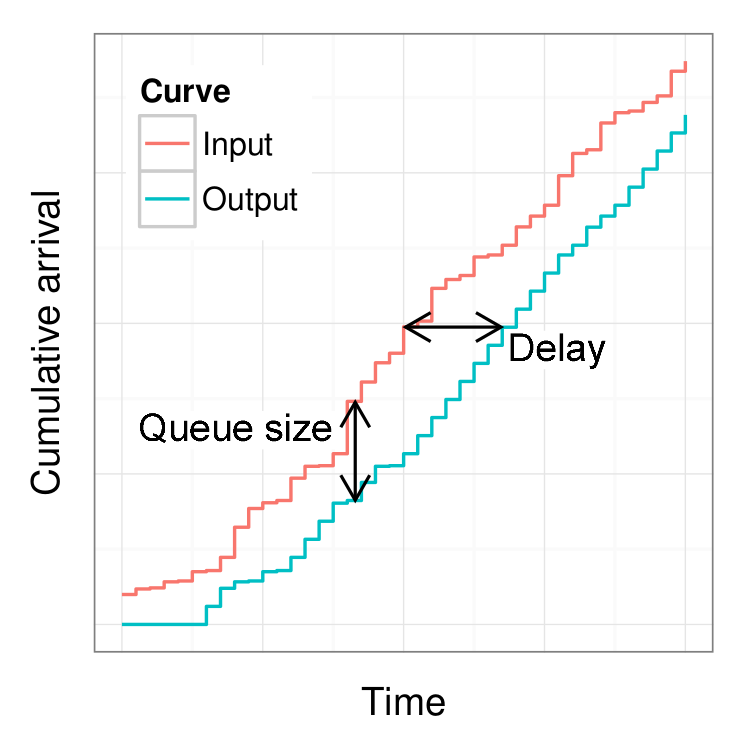
\includegraphics[width=.4\textwidth]{figures/nc_delay_and_backlog.png}
  \caption{Delay and Backlog}\label{fig:nc_delay_and_backlog}
\end{figure}

Deterministic network calculus can be used when there are no cyclic dependencies, no feedback loops, no simple analysis exists (state explosion) and when a good model of the traffic is known.

\subsection{Stochastic Network Calculus}
In stochastic network calculus flows are defined by a sequence of non-negative, real random variables $(a_n)_{n \in \mathds{N}}$ of random size.
Their cumulative arrival up to time n is then defined as $A(n) = \sum^n_{i=a}a_i$.
$(a_n)$ can follow any random distribution and are considered to be independent and identically distributed.
Similar to DNC, service curves are $S(n,m)$ of a server are defined as $A^*(n) \geq \inf_{0 \geq k \geq n} \{A(k) + S(k,n)\}$ where $S(n,m)$ can either be a stochastic or deterministic process.\\

Stochastic network calculus is mainly used for video streaming, protocols with feedback loops, wireless networks or energy networks.

\subsection{QoS in IP Networks}
In modern IP networks traffic is usually limited to a fixed set of declared parameters concerning average, peak rate and burst size.
To implement these limits, a token bucket can be used which fills with a pre-specified rate until it is full.
The limitation is then given by the cost of forwarding of one token.
To guarantee an upper bound, this approach can be combined with WFQ.

\subsubsection*{IETF Integrated Services}
The IETF integrated services provide an architecture for providing QoS guarantees in IP networks for individual application sessions.\\
If a flow/call arrives, resources have to be requested with information about the estimated traffic and reservation characteristics.
Routers then decide based on this information and remaining unreserved resources if the request can be accepted and answers accordingly.\\
Two service models are possible here.
A guaranteed service where worst-case traffic is important or a controlled load service where the QoS closely corresponds to the QoS that the same flow would receive from an unloaded network.

\subsubsection*{IETF Differentiated Services}
IEFT Differentiated Services want qualitative service classes (platinum, gold, silver services).
Implementation here differs regarding core and edge nodes.
The edge routers look at the per-flow traffic, marks packets according to a class as "in-profile" or "out-profile" and forwards to core nodes regarding a token bucket.
The core nodes then only look at the packet classes and do buffering and scheduling according to that information where "in-profile" packets have higher priority.

\subsubsection*{Classification and Conditioning}
For classification the TOS field of the IPv4 header or the Traffic class field of the IPv6 header can be used.
They consist 2 bits for a explicit congestion notification (ECN) and 6 bits that can be used for Differentiated Service Code Point (DSCP) and per hop behaviors (PHB).\\
Developed PHBs:
\begin{itemize}
  \item Expedited Forwarding: logical link with a minimum guaranteed rate.
  \item Assured Forwarding: 4 classes of bandwidth with defined guaranteed minimum bandwidth and buffering, packets can have one of three possible drop preferences
\end{itemize}

\subsection{Resource Reservation Protocol (RSVP)}
RSVP is used to communicate/signal requirements to the network.
This is done by sending information about the QoS that is required (r-spec) and the characteristics of the traffic that will be sent into the network (t-spec) to routers.\\
More precisely senders and receivers first join a multicast group.
The sender then sends a path message to make its presence known to the routers which store path states which consist of the IP address of the previous node and a sender template (data format of the sender), sender t-spec and adspec (advertisement data).
In the end of the entire communication that required RSVP, a path teardown message is sent to remove the path state from routers.\\
The receiver send a reservation message to reserve resources from sender(s) to receiver.
At every node, the destination IP changes to the next node on the reverse path and the source IP gets the address of the previous node.
In the end a reservation teardown message is sent to remove reservations.
The network only sends messages when errors occur.

\subsection{Maintaining Network State}
A state in this context is defined as information stored in network nodes by network protocols.\\
A \textbf{hard state} is installed on receiving a setup message from the sender and only removed when getting a teardown message or sometimes a heartbeat is used.
A \textbf{soft state} on the other hand is also created when receiving a setup or trigger message from the sender but is removed when the connection times out. 
For this reason a heartbeat is definitely necessary.\\
Senders in this context are nodes that (re)generate signaling messages to install, keep and remove states.
Receivers on the other hand are nodes that creates, maintains and removes states based on the messages of the sender.\\

The advantage of soft state over hard state here is that no explicit error messages need to be sent to indicate problems.
In case of a failed link the update messages will update the routes and in case of a failed host the connection will just time out.
A problem is though that if the first path message gets lost the timeout might be quite long to retry.
For that reason ACK messages can be used from receiver to sender to be able to use a quicker timeout than the normal heartbeat.

\newpage

%!TEX root = ../report.tex

\section{Node Architectures}
Nodes/Routers in a network consist of multiple input and output ports and a switching fabric in between.
There are three types of switching fabric: memory, a bus, or a crossbar (net of buses).\\
Usually the goal of a router is to completely process the incoming packets at line speed, but queuing/buffering might be necessary due to a too slow switching fabric or a overloading of one or multiple output ports.
Recommended buffer sizes are $RTT \cdot \text{link capacity}$ by RFC 3439 or $\frac{RTT \cdot \text{link capacity}} {\sqrt{\text{number of flows}}}$ more recently.\\

\textbf{First generation IP routers} had a CPU next to a global memory buffer which was connected to multiple line interfaces.
\textbf{The second generation} then introduced local memory buffers for all interfaces and the \textbf{third} moved the CPU to a separate card besides the network interfaces.
In \textbf{the forth generation} clustered and multistage network interfaces were added.

\newpage

% Needs to be enabled when there are any references.
% \clearpage
% \addcontentsline{toc}{section}{\refname}
% \printbibliography

\end{document}
